\documentclass[a4paper,12pt]{article}
\usepackage{color}
\usepackage{xcolor}
\usepackage{graphicx}
\usepackage{amsmath}
\usepackage{ulem}
\usepackage[left=1in,right=1in,top=1in,bottom=1in, headheight=15pt]{geometry}
\usepackage{setspace}
\usepackage{graphicx}
\usepackage{array}
\usepackage{cite}
\usepackage{bm}
\usepackage{float}
\usepackage{CJK}
\usepackage{indentfirst}
\usepackage{amssymb}
\usepackage[titletoc]{appendix}
\usepackage{amsfonts}
\usepackage{multirow}
\usepackage{dsfont}
\usepackage{listings} 
\usepackage{mathrsfs}
\usepackage{subfigure}
\usepackage{fancyhdr}  
\usepackage{url}
\pagestyle{fancy} 


\RequirePackage[linesnumbered,ruled,longend]{algorithm2e}
\SetKwInOut{Input}{Input}
\SetKwInOut{Output}{Output}
\newcommand{\To}{\KwTo}
\newcommand{\Ret}{\KwRet}
\SetKwProg{Fn}{Function}{\string:}{end}
\SetKw{and}{ and }
\SetKw{oor}{ or }
\SetAlTitleSty{}
\SetTitleSty{textit}{}
\newcommand{\cmt}[1]{\tcc*[f]{#1}}
\newcommand{\NULL}{{\tt NULL}}
\newcommand{\get}{\ensuremath{\gets}}

\newenvironment{Algorithm}[1][]{\def\algoname{#1}\bigskip\begin{algorithm}}{\caption{\algoname}\end{algorithm}}

\RequirePackage{ifthen}
\newcommand{\pbtype}[1]{\ifthenelse{\equal{#1}{graph}}{\def\pbtypecol{green}}{\ifthenelse{\equal{#1}{math}}{\def\pbtypecol{orange}}{\ifthenelse{\equal{#1}{combinatory}}{\def\pbtypecol{blue}}{\ifthenelse{\equal{#1}{string}}{\def\pbtypecol{red}}{\ifthenelse{\equal{#1}{network}}{\def\pbtypecol{yellow}}{\ifthenelse{\equal{#1}{ai}}{\def\pbtypecol{cyan}}{\ifthenelse{\equal{#1}{image}}{\def\pbtypecol{magenta}}{\def\pbtypecol{gray}}}}}}}}}
\newenvironment{problem}[1]{\smallskip {\bf Problem.} #1\par}{\par}

\begin{document}

\begin{titlepage}


\title{\vspace{5cm}\vspace{1cm}\textbf{Literature Research in \\
Monte Carlo Tree Search}\vspace{0.8cm}}
\author{ Liao Xinhao}
\date{\today}
\maketitle
\vspace{1cm}
\begin{center}
\begin{Large}
\textbf{Abstract}
\end{Large}\\

\end{center}

Monte Carlo Tree Search (MCTS) is a stochastic search method which is a combination of the probability statistics and the tree search method. It's based on the Monte Carlo method proposed in 1950 as an important stochastic statistic method. Proposed in 2012, MCTS is an important search method in the area of Artificial Intelligence and
has been applied to many problems. MCTS is a core algorithm of AlphaGo and has been very popular in recent years. This article mainly focuses on the theory of MCTS and some of its applications.


\thispagestyle{empty}
\end{titlepage}
\setcounter{page}{1}


\newpage

\section{Introduction}
Artificial intelligence (AI) has been a popular topic in recent years since the success of AlphaGo. Many AI technologies have been applied in AlphaGo, including the neural network, deep learning, and Monte Cralo Tree Search method. Among them, Monte Carlo Tree Search (MCTS) is a search method proposed in 2012, which has been very successful when applied to many problems. The method will be discussed in detail, and an application of MCTS will be shown. 

\section{Theoretical Background}
\subsection{Monte Carlo Method} \cite{case1}
Monte Carlo method is method used in statistics. Given a certain probability distribution, we can obtain a lot of sample results. With this idea, we can estimate an integral. Assume we have a function $f(x)$ which generates a sample result given the probability distribution of p(x), then we have
$$
{\lim_{N \to +\infty}}\frac{1}{N}\Sigma_i w_if(x_i) = \mathbb{E}_p[f(X)] $$
where $w_i$ represents the corresponding weight to $x_i$. 

It is demonstrated that using this sampling method, we can obtain some value as a reward of every move \cite{case2}.
$$
Q(s,a) = \frac{1}{N(s,a)}\Sigma_{i=1}^N(s)\mathbb{I}_i(s,a)z_i
$$
where $N(s,a)$ denotes the number of times action $a$ is selected given state $s$, and $N_s$
is the number of times ended with
state $s$.
$z_i$ is the result of the \textit{i}th simulation
starting from state $s$. $\mathbb{I}_i(s,a)$ is the identification function, which gives 1 if action $a$ is selected in state $s$, and 0 otherwise \cite{case2}.

But only sampling is not enough. A method is needed to learn from the results of sampling and then provide a reasonable estimation of the result. 
$Flat Monte Carlo$, however, provides the estimation by sampling without growing a tree\cite{case2}. Compared to MCTS, it's not a search strategy that aims to provide a promising action. 

\subsection{General MCTS Approach} 

The goal of MCTS is to estimate the expected value of action based on the Q-function given above. 
The generic MCTS algorthm is given as follows.

Here \textit{Tree Policy} covers two kinds of operations, called selection and expansion.
Selection is applied if all the children of a node is already visited and added to the tree. Then a child needs to be selected based on the values of the children. After that, \textit{Tree Policy} is recursively called given that child node.
Expansion is applied if there's a child that has not been visited. Then the tree is expanded with an added child, according to the corresponding action.

\textit{Default Policy} is to roll out a random simulation from a given state, and returns a reward value based on the simulation result. The returned reward value is later used to update the values of all nodes along the path from the root to the node where the simulation starts. That updating process is done in \textit{Backup}.



\begin{Algorithm}[General MCTS approach][H]
	% - replace nb with problem number (e.g. problem101)
% -	must match the reference in the overview
% - when writing more than one algo use problem101a, problem101b, problem101c etc.	

\Fn{MCTSSearch{($S_0$)}}{
    create root node $v_0$ with state $s_0$\\
    start tree V = \{v_0\}\\
    \While{within computation budget}{
        $v_l \leftarrow TreePolicy(V)$ 
        chooses a leaf of $V$\\
        append $v_l$ to $V$\\
        $\Delta \leftarrow DefaultPolicy(s(v_l))$
        rolls out a simulation and get the reward $\Delta$
        \\
        $Backup(v_l,\Delta)$ updates the values\\
    }
    \Ret{best child of $v_0$}
}	

\end{Algorithm}

Fig. 1 below shows how the general MCTS approach works \cite{case2}.

\begin{figure}[H]
    \centering
    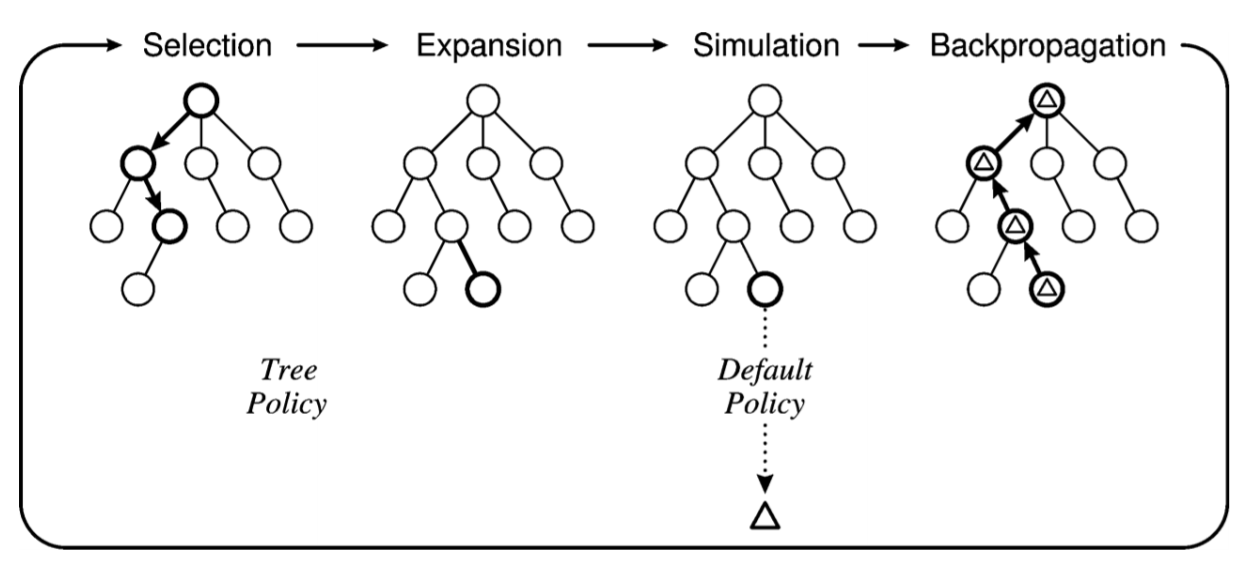
\includegraphics[width = 15cm]{MCTS.png}
    \caption{The general MCTS approach}
\end{figure}


\subsection{Upper Confidence Bounds for Trees (UCT)} 

MCTS evaluate the values of nodes and iteratively build a partial search tree \cite{case2}. Notice that for the \textit{Tree Policy}, selection is made to choose the next action given the learned knowledge of values obtained from the simulation. The problem is how the child node is selected. Not only the value, which is the accumulation of the reward of simulations, but also the number of times of simulations needed to be taken into account. This is because of the exploitation-exploration dilemma: 
the currently optimal exploitation needs to be balanced with the exploration of other actions, that might turn out to generate a better result \cite{case2}. Hence, for each node $v$ in the search tree, it should hold 2 values, that is, $Q(v)$ for the values that is the total rewards accumulated, and $N(v)$ is the number of times it has been visited \cite{case2}.


``Upper Confidence Bounds (UCB)" is an evaluation 
that tells how much a selection is potentially to be optimal, which is used to address the exploitation-exploration dilemma. UCB1 is the simplest UCB policy, which is widely used \cite{case3}. It is given as
$$
 UCB1 = \overline{X_j} + \sqrt{\frac{2\text{ln}n}{n_j}}
$$
where $\overline{X_j}$ is the average value per visited time for the $j$th child node, which is $\frac{Q(v_j)}{n_j}$, $n$ represents the number of times the parent node is visited, and $n_j$ is the number of times the $j$th child is visited \cite{case2}.

UCT uses UCB1 to realize \textit{Tree Policy}, and is given below
$$
 UCT = \overline{X_j} + 2C_p\sqrt{\frac{2\text{ln}n}{n_j}}
$$
where $\overline{X_j}$ is the average value per visited time for the $j$th child node, which is $\frac{Q(v_j)}{n_j}$, $n$ represents the number of times the parent node is visited, and $n_j$ is the number of times the $j$th child is visited , and $C_p$ is a cnostant which can be adjusted to affect the exploration decision \cite{case2}. The child $j$ is selected to maximize this value.
For the rewards set to be in the range of [0,1], the constant $C_p$ should be set to $\frac{1}{\sqrt{2}}$ for a better result \cite{case4}. 

Using UCT, the MCTS algorithms can be completed as follows \cite{case2}.


\begin{Algorithm}[Tree Policy][H]
	% - replace nb with problem number (e.g. problem101)
% -	must match the reference in the overview
% - when writing more than one algo use problem101a, problem101b, problem101c etc.	
\Fn{TreePolicy{($v$)}}{
	\While{$v$ not terminal}{
	    \If{$v$ not fully expanded}
	        {\Ret{Expand($v$)}}
	    \Else{
	        v\leftarrow BestChild(v,C_p)\\
	        }
	}
	\Ret{$v$}
}
\end{Algorithm}

\begin{Algorithm}[Expand][H]
	% - replace nb with problem number (e.g. problem101)
% -	must match the reference in the overview
% - when writing more than one algo use problem101a, problem101b, problem101c etc.	
\Fn{Expand{($v$)}}{
    choose $s' \in $  states corresponding untried actions in $A(s(v))$\\
    add a new child $v'$ to $v$ such that $s(v') = s'$\\
	\Ret{$v'$}
}
\end{Algorithm}

\begin{Algorithm}[Best Child][H]
	% - replace nb with problem number (e.g. problem101)
% -	must match the reference in the overview
% - when writing more than one algo use problem101a, problem101b, problem101c etc.	
\Fn{BestChild{($v$, $c$)}}{
	\Ret{$\mathop{\arg\max}_{v' \in \text{children of} \ v} \frac{Q(v')}{N(v')} + c\sqrt{\frac{2\text{ln}N(v)}{N(v')}}$ }
}
\end{Algorithm}

\begin{Algorithm}[Default Policy][H]
	% - replace nb with problem number (e.g. problem101)
% -	must match the reference in the overview
% - when writing more than one algo use problem101a, problem101b, problem101c etc.	
\Fn{DefaultPolicy{($s$)}}{
	\While{$s$ not terminal (and within the time limit)}{choose the next possible state $s'$ randomly\\
	    s \leftarrow s'\\
	    }
	\Ret{reward of state $s$}}
\end{Algorithm}

\begin{Algorithm}[Back Up][H]
	% - replace nb with problem number (e.g. problem101)
% -	must match the reference in the overview
% - when writing more than one algo use problem101a, problem101b, problem101c etc.	
\Fn{BackUp{($v$, $\Delta$)}}{
	\While{$v$ not NULL}
	    {$N(v)\leftarrow N(v)+1$\\
	    $Q(v)\leftarrow Q(v) + \Delta$\\
	    $v\leftarrow$ parent of $v$}
}
\end{Algorithm}


\section{Application Cases}

Board games have long been used to test the algorithms in AI. The success of AlphaGo, which uses MCTS as an important component, in October 2015 has shown the power of this algorithm, along some many other important technologies in AI, like neural network and deep learning. MCTS is widely applied to many games, especially board games like $Go$. The figure below shows such an example, named \textit{Clickomania} or \textit{SameGame}  \cite{case5}.

\begin{figure}[H]
    \centering
    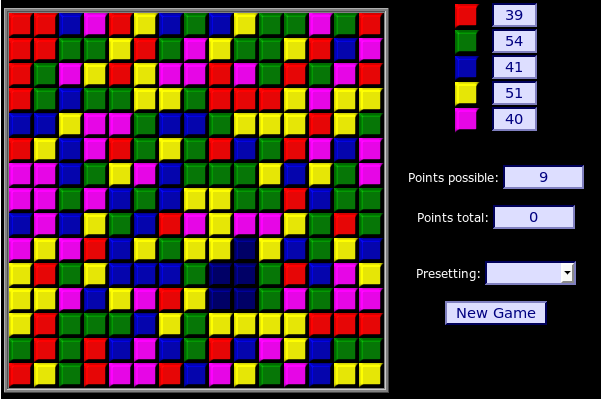
\includegraphics[width = 10cm]{SameGame.png}
    \caption{An initial state of the SameGame problem}
\end{figure}

\textit{SameGame} is a popular puzzle game
which aims to clear the coloured blocks. The consecutive blocks with the same colour can be cleared in one action, and
scores will be obtained based on the number of squares $n$ cleared in one action, which is usually $(n-2)^2$ \cite{case5}. So for MCTS, the reward for one simulation can be easily set based on the obtained score of the simulation result.
In \cite{case5}, an Monte Caro Search heuristic called \textit{Nested Rollout Policy Adaptation} (NRPA) and the parallel architecture is used along with MCTS to address the SameGame problem. 

Besides many game applications, MCTS can also be applied to many non-game problems. For instance,
MCTS has been used to address Traveling Salesman Problem (TSP) in \cite{case6}. 
In general, MCTS is very promising in many
nongame applications, in areas of planning, scheduling, optimization,
and a range of other decision domains \cite{case2}.






\section{Discussion and Conclusion}

MCTS, proposed within 10 years, is actually a very new algorithm in the area of AI. By ``combining the precision of tree search with the generality
of random sampling", MCTS is able to provide good enough results after sampling and learning \cite{case2}. It can be efficient given appropriate search heuristic based on the problem. 

Trace back to the origin of MCTS, Monte Carlo method has been invented for over 60 years. It's not a complex idea at all.
However, it had never been as popular as it is now. The reason is that the precision of this method depends largely on the number of sampling times. 
With the development of electronic and computer technology in the past decades, it has now become a very powerful method in the area of AI, and has made incredible success in recent years. 

Science and technology are rapidly changing these day. Many old mainstreams are being deserted, and some abandoned ideas, like Monte Carlo method, are being rediscovered. What is a good idea? It actually doesn't need to be complex, or even sound feasible. Just as Geoffrey Hinton, the ``godfather of deep learning" said, ``read enough so you start developing intuitions. And then, trust your intuitions and go for it"\cite{case7}.

\begin{thebibliography}{0}

\bibitem{case1}
B. Abramson, ``Expected-outcome: A general model of static evaluation," IEEE Trans. Pattern Anal. Mach. Intell., vol. 12, no. 2, pp.182–193, Feb. 1990


\bibitem{case2}
C. B. Browne et al., ``A Survey of Monte Carlo Tree Search Methods," in IEEE Transactions on Computational Intelligence and AI in Games, vol. 4, no. 1, pp. 1-43, March 2012.
doi: 10.1109/TCIAIG.2012.2186810

\bibitem{case3}
 P. Auer, N. Cesa-Bianchi, and P. Fischer, ``Finite-time analysis of the
multiarmed bandit problem," Mach. Learn., vol. 47, no. 2, pp. 235–256,
2002.

\bibitem{case4}
L. Kocsis, C. Szepesvári, and J. Willemson, ``Improved Monte-Carlo
search," Univ. Tartu, Tartu, Estonia, Tech. Rep. 1, 2006

\bibitem{case5}
Negrevergne, Benjamin , and T. Cazenave . ``Distributed Nested Rollout Policy for SameGame." 2017.

\bibitem{case6}
A. Rimmel, F. Teytaud, and T. Cazenave, ``Optimization of the nested
Monte-Carlo algorithm on the traveling salesman problem with time
windows," in Proc. Appl. Evol. Comput. 2, Torino, Italy, 2011, pp.
501–510.

\bibitem{case7}
 ``Geoffrey Hinton interview", https://www.coursera.org/learn/neural-networks-deep-learning/lecture/dcm5r/geoffrey-hinton-interview

\end{thebibliography}


\end{document}